\section{LHCb Overview}

The main aim of the LHCb experiment is to study CP violation processes and other rare phenomena particularly those involving the decay of  B and D mesons. Designed to build upon the research carried out by the B factories Belle and BarBar, LHCb aims to produce significant improvements on the available statistics of $B^+$, $B^0$ and $B_s$ decays. This enables LHCb to further constrain and confirm results from the B factories as well as investigate the possibilities of new physics.

The requirements for the detector include high precision vertex resolution is required to identify secondary vertices and tag $B$ events; accurate particle identification is required to detect and classify rare processes; and a fast and efficient trigger with the ability to filter the copious events produced from the LHC's high luminosity.

The LHCb detector is a single arm spectrometer with a forward angular coverage from approximately 10 mrad to 300 [250] mrad in the bending [non-bending] plane. It comprises of a vertex detection system, a tracking system, Ring Imaging Cherenkov Detectors (RICH), a calorimeter system, muon detector, trigger system and computing farm. Each have been specifically designed to achieve the criteria stated previously and individually discussed in the following sections.

\begin{figure}
	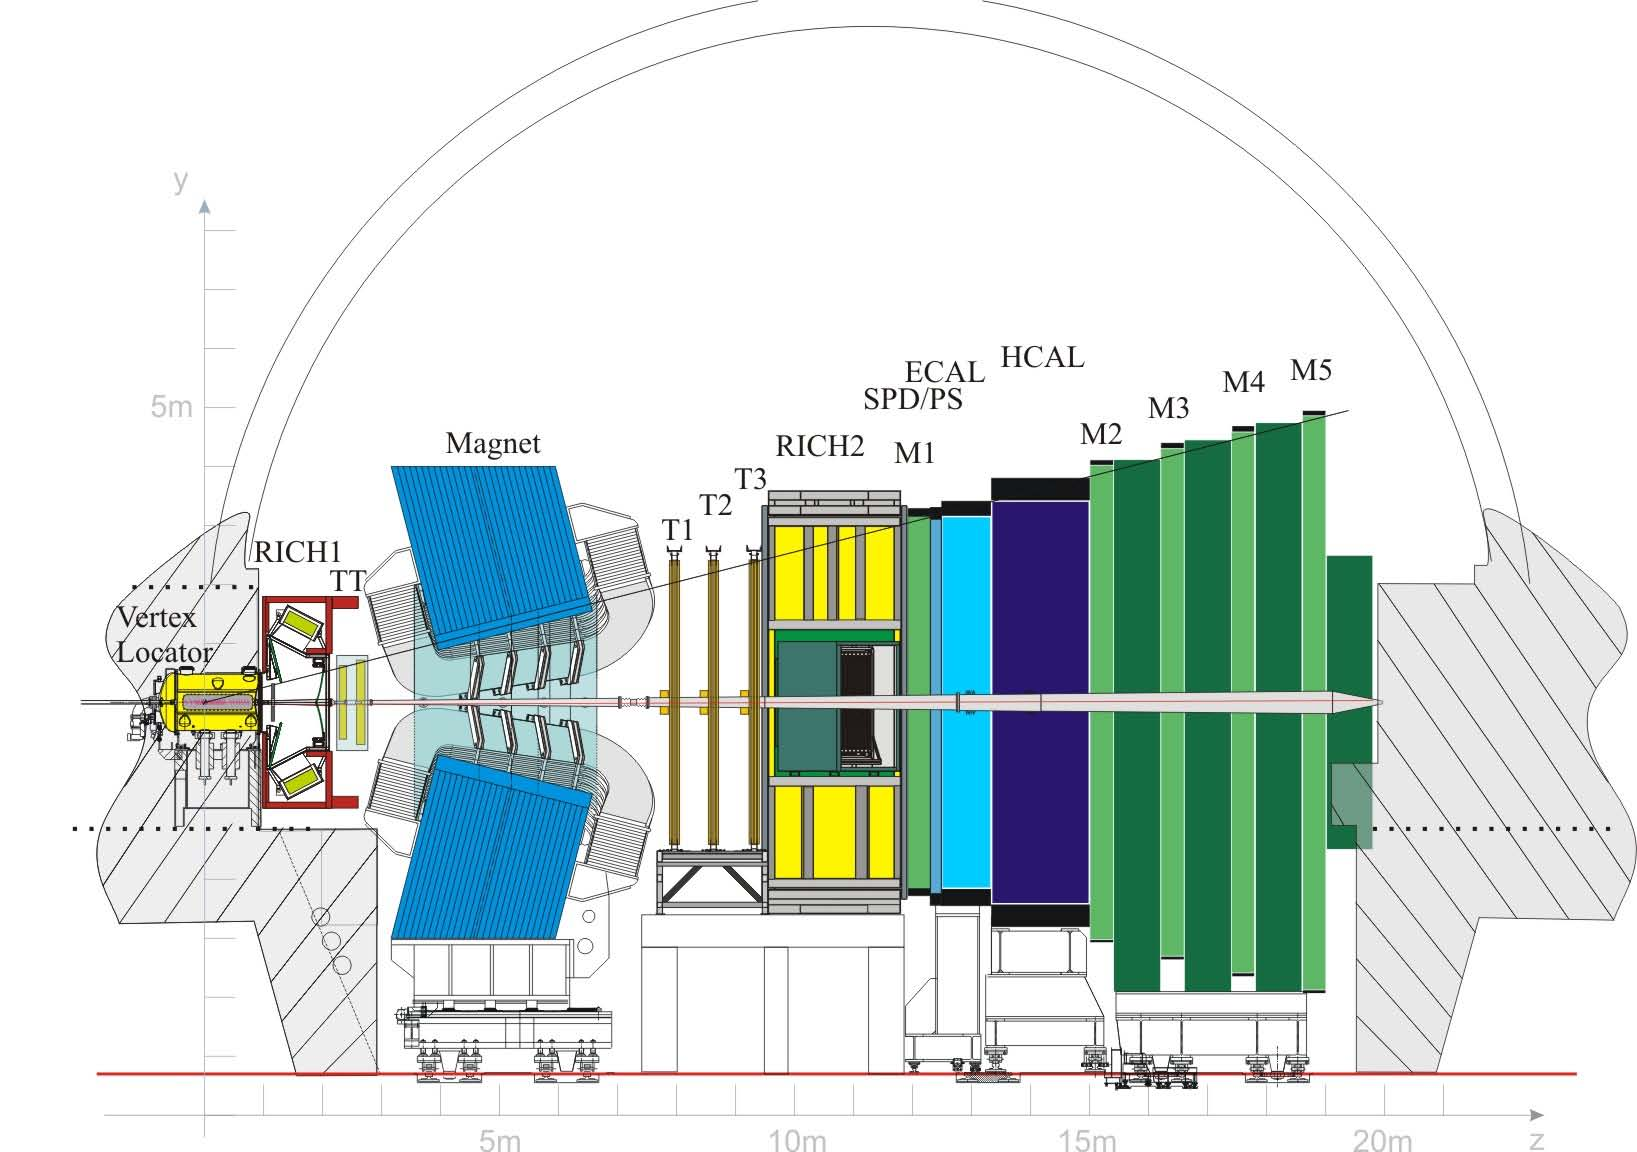
\includegraphics[width=\columnwidth]{Chapters/detector/images/lhcb_schematic.jpg}
	\caption{LHCb schematic}
	\label{fig: lhcb_schematic}
\end{figure}

% DETECTOR ACEPTANCE
%Figure \ref{} shows the momentum distribution for $\pi^+ \pi^-$ pairs from the decay of $B_d^0$ particles. Overlaid are $\pi^+ \pi^-$ pairs which have been reconstructed within the LHCb detector and $\pi^+ \pi^-$ pairs that have not. Events are produced by the PYTHIA event generator.  The decrease in detector acceptance at low momenta is due to slow pions that do not hit enough tracking stations for their momenta to be measured. This is due to the magnet bending the path of low momenta pions outside the detector acceptance. At high momenta the decrease in detector acceptance is due to particles with trajectories that are within the beam pipe.
